\documentclass[11pt,a4paper]{article}
\usepackage[T1]{fontenc}
\usepackage[utf8]{inputenc}
\usepackage{lmodern,microtype}
\usepackage{amsmath,amssymb,amsthm,mathtools,bm}
\usepackage{booktabs,array,tabularx,longtable}
\usepackage{graphicx,float,caption}
\usepackage{xcolor}
\usepackage[margin=21mm]{geometry}
\usepackage{enumitem}
\usepackage{fancyhdr}
\usepackage[hidelinks]{hyperref}
\hypersetup{
  pdftitle={FIN jako hipotetyczna Teoria Wszystkiego: Atlas Cieni Znanych Teorii Fizycznych},
  pdfauthor={Krzysztof Żuchowski},
  pdfsubject={Kontrfaktyczna analiza znanych teorii jako efektywnych projekcji FIN},
  pdfkeywords={FIN, teoria wszystkiego, teoria operatorów, mechanika kwantowa, QFT, grawitacja, informacja, renormalizacja, solitony}
}
\setlength{\parindent}{0pt}
\setlength{\parskip}{0.52em}
\setlength{\emergencystretch}{2em}
\setlength{\headheight}{14pt}
\setlist[itemize]{leftmargin=1.6em,itemsep=0.18em,topsep=0.2em}
\setlist[enumerate]{leftmargin=1.8em,itemsep=0.18em,topsep=0.2em}
\pagestyle{fancy}
\fancyhf{}
\lhead{FIN --- Atlas Cieni Teorii Fizycznych}
\rhead{Release 10.54}
\cfoot{\thepage}
\newtheorem{theorem}{Twierdzenie}[section]
\newtheorem{proposition}[theorem]{Propozycja}
\newtheorem{corollary}[theorem]{Wniosek}
\newcommand{\proven}{\textcolor{green!45!black}{\textbf{[UDOWODNIONE]}}}
\newcommand{\strong}{\textcolor{blue!70!black}{\textbf{[MOCNE DOWODY]}}}
\newcommand{\conditional}{\textcolor{black!60}{\textbf{[WARUNKOWE]}}}
\newcommand{\analogy}{\textcolor{orange!85!black}{\textbf{[ANALOGIA]}}}
\newcommand{\absent}{\textcolor{red!72!black}{\textbf{[BRAK MOSTU]}}}
\newcommand{\claimbox}[1]{\begin{center}\fcolorbox{blue!60!black}{blue!4}{\parbox{0.92\textwidth}{#1}}\end{center}}
\renewcommand{\contentsname}{Spis treści}
\renewcommand{\refname}{Literatura}

\begin{document}

\pagenumbering{gobble}
\begin{titlepage}
\centering
\vspace*{1.7cm}
{\LARGE\bfseries FIN jako hipotetyczna Teoria Wszystkiego\par}
\vspace{0.55cm}
{\Large Atlas Cieni Znanych Teorii Fizycznych\par}
\vspace{0.5cm}
{\large Jak równania opisujące obserwowane zjawiska mogłyby być efektywnymi objawami jednego informacyjno-spektralnego fundamentu\par}
\vspace{1.45cm}
{\Large Krzysztof Żuchowski\par}
\vspace{0.28cm}
{\large Independent Researcher --- Fractal Information Theory Project\par}
{\large ORCID: 0009-0002-0909-3613\par}
\vspace{1.25cm}
{\large FIN Release 10.54 --- Version 1.0.0\par}
{\large 10 sierpnia 2026\par}
\vfill
\begin{minipage}{0.86\textwidth}
\textbf{Założenie badawcze.} Raport przyjmuje kontrfaktycznie hipotezę $H_{\rm TOE}$: FIN jest mikroskopowym fundamentem rzeczywistości, a znane teorie są jego sektorami efektywnymi, projekcjami lub fenomenologicznymi cieniami. Hipoteza organizuje porównanie; nie zmienia statusu żadnego istniejącego dowodu.\par
\textbf{Metoda.} Połączono audyt aktualnego rdzenia FIN dostępnego w lokalnym snapshotcie, obliczenia dla ścisłego operatora, kontrolę zerową na $10\,000$ próbkowanych dodatnich laplasjanach cyrkulantowych oraz porównanie z literaturą pierwotną, w szczególności z arXiv i źródeł DOI. Bazowy Git HEAD: \texttt{35b2d58ebde7103cc68c77e84620e24d6c058de2}; drzewo zawierało jawne lokalne artefakty poza commitem.\par
\textbf{Granica.} Raport nie ogłasza FIN teorią fizycznie potwierdzoną. Rozróżnia dokładną tożsamość matematyczną, realizację warunkową, analogię i brak mostu. Nie przenosi historycznych ról legacy na strict.\par
\textbf{Repozytorium.} \url{https://github.com/hyconiek/Fractal-Nadsoliton-Theory}\par
\textbf{Licencja.} CC BY 4.0.
\end{minipage}
\end{titlepage}
\pagenumbering{arabic}

\begin{abstract}
Przyjęcie, że FIN jest teorią fundamentalną, pozwala postawić precyzyjne pytanie odwrotne: które znane równania fizyki można otrzymać jako różne sposoby obserwacji, redukcji lub rachunku funkcyjnego jednego obiektu FIN? Najsilniejsza odpowiedź dotyczy dodatniego samosprzężonego generatora
\[
 W_{xx}=0,\quad W_{xy}=K_{\rm strict}(d(x,y))\ (x\ne y),\qquad
 A=sI-W\succeq0,\qquad
 A=\sum_r\lambda_rE_r.
\]
Dokładnie te same $\lambda_r$ i $E_r$ generują fazy $e^{-it\lambda_r}$, relaksacje $e^{-t\lambda_r}$, odpowiedź Greena $(\lambda_r+z)^{-1}$, dynamikę falową $\cos(t\sqrt{\lambda_r})$ i formalne wagi Gibbsa $e^{-\beta\lambda_r}/Z$. Są to dokładne \emph{transformacje spektralne} jednego operatora i kandydaci na cienie fizyczne. Cieniami fizycznymi stają się dopiero po skonstruowaniu pełnych map sektora, jednostek, coarse grainingu oraz pomiaru.

Obliczenie rekonstruuje wspólne widmo z czterech transformacji z błędami $2.2\times10^{-16}$--$4.4\times10^{-15}$, przy jawnie znanym przedziale widma i ustalonym modzie zerowym. Semigrupa $e^{-0.55A}$ ma wszystkie elementy dodatnie, sumy wierszy i kolumn równe jeden do $4.4\times10^{-16}$ oraz szczegółową równowagę. Zarazem jednooperatorowa algebra $C^*(A)$ ma tylko siedem wymiarów wobec $144$ wymiarów pełnej algebry macierzy i jest przemienna. Każde $f(A)$ zachowuje translacje oraz odbicie. Z samego $C^*(A)$ nie można więc uzyskać nieprzemiennej algebry obserwabli, CCR/CAR, nieabelowej krzywizny cechowania ani selektora orientacji; nie jest to no-go dla rozszerzeń zawierających dodatkową algebrę lub generator.

Kontrola zerowa testuje specyficzność, nie prawdziwość FIN. Wszystkie $10\,000$ prób z jednej jawnej miary lognormalnej na dodatnich radialnych wagach $C_{12}$ posiadały wspólny rachunek funkcyjny i dodatnią semigrupę Markowa; w tej klasie wynik wynika także analitycznie z własności laplasjanu. Percentyle zależą od wybranej miary (typowy błąd Monte Carlo wynosi około $0.3$--$0.5$ punktu procentowego). Ścisłe widmo ma mierzalną strukturę --- między innymi znormalizowana luka leży na $10.12$ percentylu, a liczba uwarunkowania na $86.62$ --- lecz żaden z pięciu wskaźników nie jest ekstremalny na poziomie jednego procenta w tym zespole.

Raport klasyfikuje reprezentatywny, niewyczerpujący wybór osiemnastu dziedzin. Skończona teoria operatorów, proces Markowa, Green i gaussowska eliminacja Schura mają najbliższe dokładne odpowiedniki matematyczne. Mechanika kwantowa, statystyka, układy otwarte i DNLS są realizacjami warunkowymi. Pełna QFT, hydrodynamika, geometria nieprzemienna i tensor networks pozostają analogiami wymagającymi nowych struktur. Yang--Mills, Model Standardowy, ogólna teoria względności i causal sets nie są obecnie wyprowadzone.

Najbardziej falsyfikowalną wersją hipotezy jest węższy ansatz $H_{1A}$: wybrane kanały są funkcjami jednego zamrożonego $A$. Jeżeli niezależnie zrekonstruowane częstości, szybkości relaksacji, bieguny odpowiedzi i wagi termiczne nie mają wspólnej dopuszczalnej klasy generatora, upada $H_{1A}$, nie ogólne i niedookreślone $H_{\rm TOE}$. Najmniejsza kandydacka TOE musi rozszerzyć pojedynczy operator do operacyjnego systemu spektralnego zawierającego algebrę obserwabli, stan, sektory, jednostki, refinację, instrumenty, środowisko i rekord.
\end{abstract}

\textbf{Słownik statusów.} \proven{} oznacza twierdzenie lub dokładny wynik obliczeniowy w zadanym modelu; \strong{} --- odporny wynik numeryczny; \conditional{} --- wynik po dodaniu jawnych struktur; \analogy{} --- podobieństwo bez diagramu redukcji; \absent{} --- brak wymaganej mapy lub sprzeczność typów. Kody E oznaczają rodzaj relacji: E1 --- dokładna tożsamość matematyczna w modelu skończonym; E2 --- realizacja warunkowa po dodaniu jawnych obiektów; E3 --- analogia strukturalna bez diagramu redukcji; E0 --- brak mostu lub niezgodność typów. Poziomy L mierzą osobno dojrzałość redukcji fizycznej.

\tableofcontents
\newpage

\section{Pytanie, które raport rzeczywiście rozstrzyga}

Hipoteza robocza ma postać
\begin{equation}
 H_{\rm TOE}:\qquad \text{FIN jest fundamentem, a znane teorie opisują jego efektywne objawy.} \label{eq:htoe}
\end{equation}
Jest to hipoteza kontrfaktyczna i obecnie niedookreślona. Jej testowalnym podprzypadkiem jest
\begin{equation}
 H_{1A}:\qquad U_t,\ P_t,\ G_z,\ C_t\ \text{i}\ \rho_\beta
\text{ są funkcjami jednego, niezmienionego generatora }A,                 \label{eq:h1a}
\end{equation}
z uprzednio zarejestrowanym, skończonym zestawem kanałowych map skal. Nie pytamy, czy znane teorie można nazwać językiem FIN. Pytamy, czy istnieją mapy, które z dynamiki FIN wytwarzają ich stany, symetrie, równania, obserwable i parametry.

Znana teoria $T$ jest cieniem FIN, jeśli można skonstruować diagram
\begin{equation}
(\mathcal S_{\rm FIN},\Phi_\tau,G_{\rm FIN})
\xrightarrow{\Sigma_T}
\mathcal S_{\rm FIN}^{(T)}
\xrightarrow{D_T}
\widetilde{\mathcal S}_T
\xrightarrow{C_{\Lambda,T}}
(\mathcal S_T,\Psi_t,G_T)
\xrightarrow{M_T}
\operatorname{Prob}(\mathcal R_T).                 \label{eq:shadowdiagram}
\end{equation}
Tutaj $\Sigma_T$ wybiera sektor lub próżnię, $D_T$ nadaje jednostki, $C_{\Lambda,T}$ wykonuje coarse graining albo limit kontinuum, a $M_T$ definiuje przygotowanie, instrument, aparat i rekord.

Dla kontrolowanego limitu musi zachodzić przeplatanie
\begin{equation}
C_{\Lambda,T}D_T\Sigma_T\Phi_\tau
=\Psi_{t(\tau)}C_{\Lambda,T}D_T\Sigma_T+R_{\Lambda,T},
\qquad \|R_{\Lambda,T}\|\longrightarrow0.          \label{eq:intertwine}
\end{equation}
Każda obserwabla $O_T$ wymaga pullbacku $J_T(O_T)$ i kontroli błędu oczekiwania. Bez tych map wzór może być dokładną transformacją matematyczną, ale nie jest jeszcze cieniem fizycznym ani wyprowadzeniem teorii $T$.

\subsection{Poziomy siły związku}

\begin{center}
\small
\begin{tabularx}{\textwidth}{@{}p{0.07\textwidth}p{0.20\textwidth}X@{}}
\toprule
Poziom & Nazwa & Kryterium\\
\midrule
L0 & analogia & Podobny wzór lub zachowanie bez mapy redukcji.\\
L1 & reprezentacja & Obiekt teorii można zapisać przez FIN, lecz semantyka i parametry są dostarczone.\\
L2 & emulacja & FIN odtwarza zadane trajektorie lub rekordy w skończonym teście.\\
L3 & limit efektywny & Istnieje rodzina refinacji i dowód $\|R_{\Lambda,T}\|\to0$.\\
L4 & wyprowadzenie & Symetrie, skale, obserwable i parametry wynikają z FIN i jawnie minimalnych aksjomatów.\\
L5 & potwierdzenie & Nowa niezależna predykcja przechodzi zewnętrzny test fizyczny.\\
\bottomrule
\end{tabularx}
\normalsize
\end{center}

Lokalne badania mogą dowieść formalnych składników wymaganych przez L4, lecz sama identyfikacja ich znaczenia fizycznego nie może zostać potwierdzona bez zewnętrznego rekordu. Syntetyczny eksperyment, wykres podwójnej szczeliny lub symulowany detektor nie są L5.

\section{Co przyjmujemy jako FIN}

Ontologicznym punktem startu jest jeden nadsoliton: pierwotna samopodobna informacja w trwałym stanie solitonicznym, bez niższej warstwy informacyjnej. Preferowany porządek programu to
\[
\text{nadsoliton}\longrightarrow\text{światło}\longrightarrow\text{materia}\longrightarrow\text{obserwator emergentny}.
\]
Jest to $H_{\rm TOE}$, a nie rezultat pomiaru.

Najmniejszym udowodnionym rdzeniem jest natomiast skończony nośnik $C_{12}$, ścisły profil
\[
K_{\rm strict}(d)=\frac{\cos(0.18575d+0.16250)}{1+d^{9/5}},
\]
macierz $W$ o zerowej przekątnej, $W_{xy}=K_{\rm strict}(d(x,y))$ dla $x\ne y$, i laplasjan
\[
A=sI-W,\qquad s=1.660307278766099,\qquad
\langle f,Af\rangle=\frac12\sum_{x,y}W_{xy}|f_x-f_y|^2\ge0.
\]

Historyczny
\[
K_{\rm legacy,ont}(d)=\alpha_{\rm geo}
\frac{\cos(\pi d/4+\pi/6)}{1+\beta_{\rm tors}d}
\]
pozostaje pośrednim jądrem mostowym. Nie jest cichym substytutem strict. W ograniczonym diagnostyku kształtu (kanoniczna faza, $\log\beta\in[-12,8]$, swobodna także znakowo amplituda, nieważona norma euklidesowa sześciu odległości $d=1,\ldots,6$) najniższy znaleziony względny residual wynosi $0.99126$ i leży blisko brzegu $\beta\to0$; dla $\beta_{\rm tors}=0.01$ wynosi $0.99148$. Nie uwzględnia to krotności Frobeniusa $2,2,2,2,2,1$ i nie jest dowodem globalnego optimum fizycznie dopuszczalnej rodziny. Wynik nie tworzy mapy completion ani twierdzenia role-transfer.

Stary diagram $K_{\rm geo}K_{\rm res}(1+0.2K_{\rm tors})K_{\rm topo}$ zachowuje wartość jako generator intuicji: tłumienie, rezonans, faza i wielościeżkowość to rozsądne klasy mechanizmów. Nie jest dowodem hydrodynamiki, cechowania lub topologicznego tunelowania. Zawiera również wykryte błędy arytmetyczne i niepoprawny wzór węzłów, dlatego jego dawne deklaracje ``pomiarów Wilsona'' nie są używane jako dane.

\section{Twierdzenie o wspólnej transformacji spektralnej}

Niech
\[
A=\sum_r\lambda_rE_r.
\]
Wtedy rachunek funkcyjny daje
\begin{align*}
U_t&=e^{-itA}=\sum_re^{-it\lambda_r}E_r,\\
P_t&=e^{-tA}=\sum_re^{-t\lambda_r}E_r,\\
G_z&=(A+zI)^{-1}=\sum_r(\lambda_r+z)^{-1}E_r,\\
C_t&=\cos(t\sqrt A)=\sum_r\cos(t\sqrt{\lambda_r})E_r,\\
\rho_\beta&=\frac{e^{-\beta A}}{\operatorname{tr}e^{-\beta A}}
=\sum_r\frac{e^{-\beta\lambda_r}}{Z}E_r.
\end{align*}

\begin{theorem}[Wspólna rodzina transformacji]
Jedna dodatnia samosprzężona macierz generuje dokładnie spójną rodzinę transformacji unitarnych, cieplnych, falowych, odpowiedzi Greena i formalnych stanów Gibbsa. Wszystkie mają te same projektory spektralne; różnią się wyłącznie funkcją zastosowaną do wspólnych wartości własnych. Twierdzenie nie nadaje tym transformacjom semantyki fizycznej.
\end{theorem}

W zamkniętym teście round-trip wygenerowano macierze z strict $A$, po czym odtworzono ich widma z $P_{0.55}$, $G_{0.70}$, $U_{0.55}$ i $\rho_{0.80}$ z maksymalnymi błędami odpowiednio $3.89\times10^{-15}$, $4.44\times10^{-15}$, $2.22\times10^{-16}$ i $2.22\times10^{-16}$. Dla $U_t$ użyto znanego przedziału widma oraz gałęzi bez aliasingu: $t\lambda_{\max}=1.288<\pi$ i $\lambda_{\min}=0$. Stan Gibbsa określa tylko różnice $\lambda_r-\lambda_0$; normalizację ustala mod zerowy, a rekonstrukcja projektorów wymaga tomografii całej macierzy, nie samych wag. Jest to test spójności implementacji i algebry, nie niezależna rekonstrukcja kanału ani ślepa identyfikacja eksperymentalna. Wszystkie dziesięć komutatorów pomiędzy $A,U,P,G,C$ ma normę poniżej $2.82\times10^{-15}$.

\begin{figure}[H]
\centering
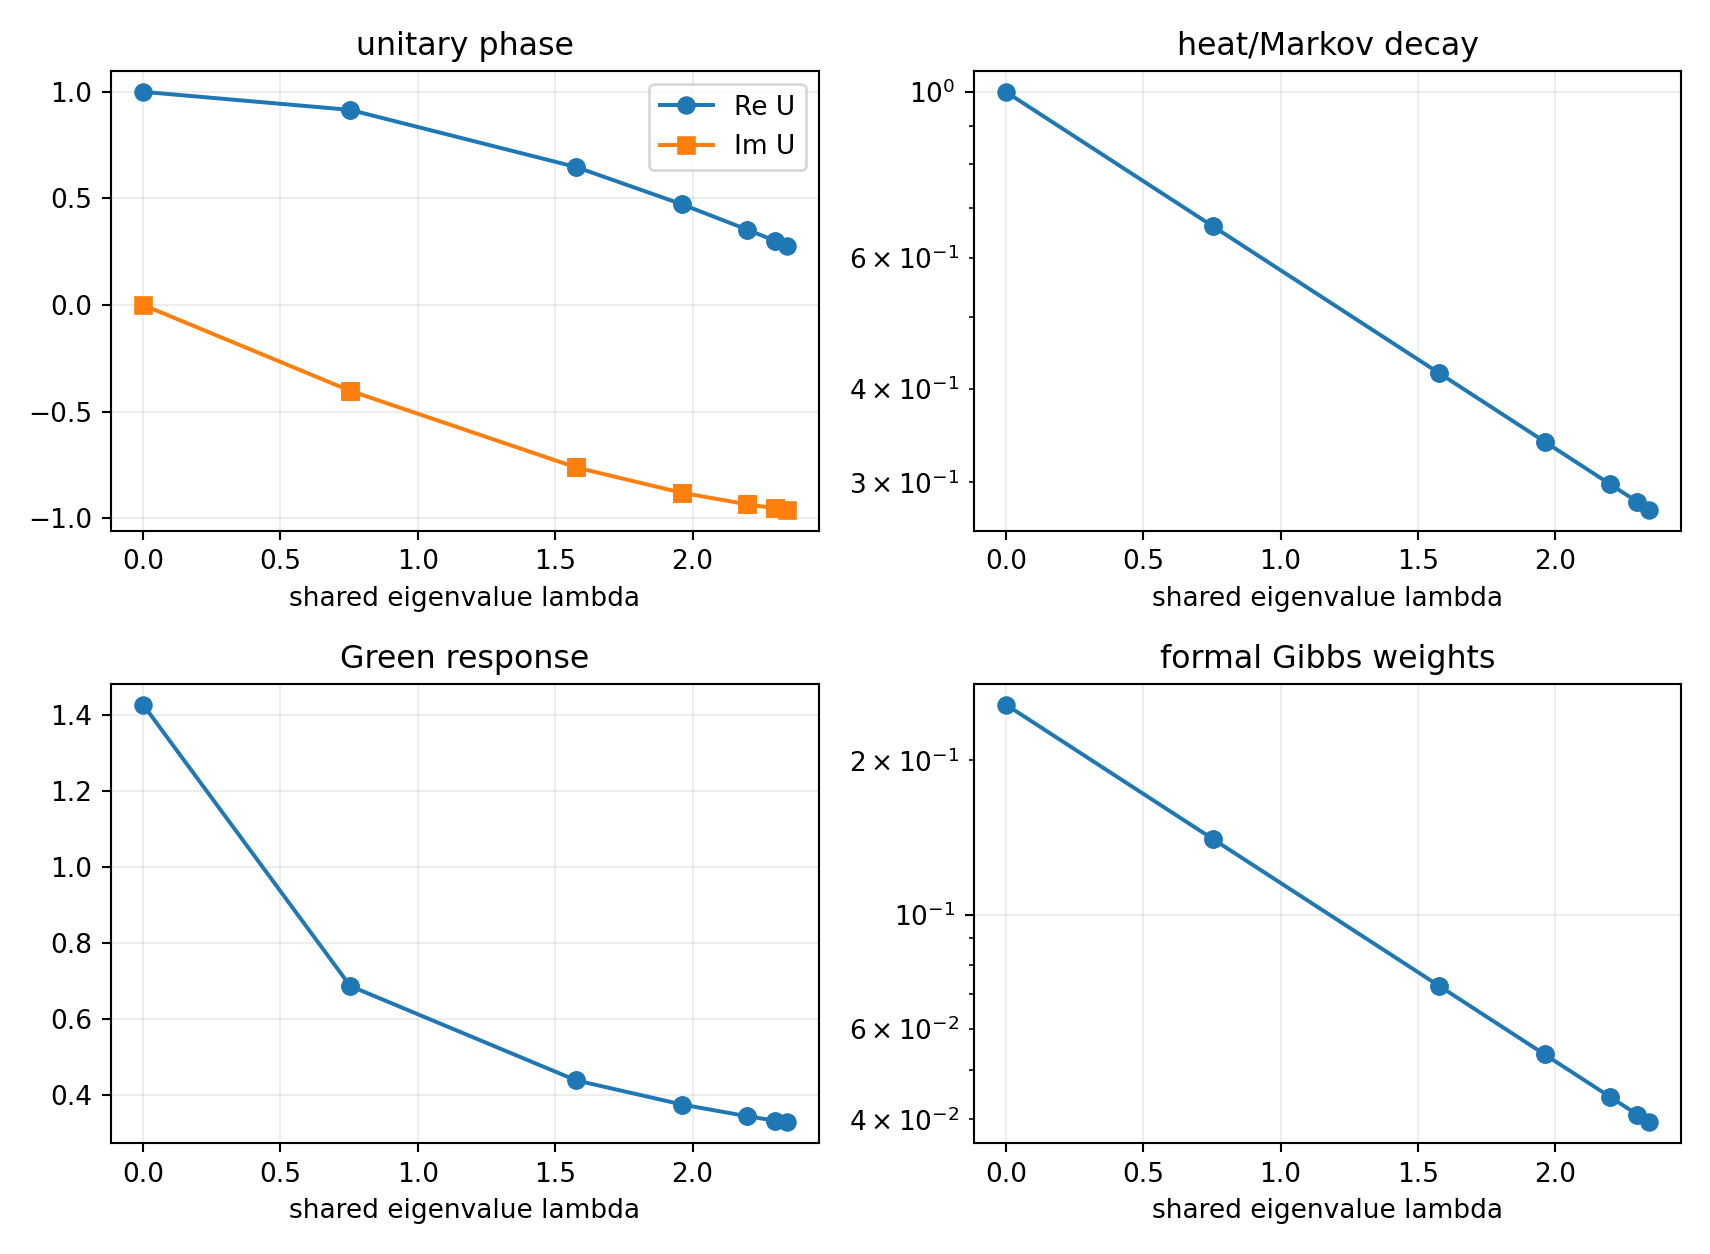
\includegraphics[width=0.90\textwidth]{FIN_TOE_Shadow_Atlas_Figures/common_spectrum_four_shadows.png}
\caption{Cztery transformacje są funkcjami tych samych wartości własnych. Jest to ścisła unifikacja matematyczna; identyfikacja fizyczna pozostaje osobnym problemem.}
\end{figure}

\subsection{Najsilniejszy wspólny test fizyczny}

Jeżeli obowiązuje wąski ansatz $H_{1A}$, to po zamrożeniu małej liczby kanałowych skal transformacje muszą dawać tę samą dopuszczalną klasę $\lambda_r$ i $E_r$:
\begin{center}
$\omega_{U,r}\propto\lambda_r\ \leftrightarrow\ \gamma_{P,r}\propto\lambda_r
\ \leftrightarrow\ \omega_{C,r}^{2}\propto\lambda_r
\ \leftrightarrow\ $ bieguny Greena $\ \leftrightarrow\ -\log(p_r/p_0)\propto\lambda_r-\lambda_0$.
\end{center}
Nie porównuje się więc surowej częstości falowej $\sqrt{\lambda_r}$ z szybkością relaksacji $\lambda_r$. Jedno ustalone przypisanie wymiaru operatorowi $A$ nie może czynić go jednocześnie generatorem o wymiarze $1/t$ i sztywnością o wymiarze $1/t^2$ bez jawnych map sektorowych.
Oddzielne dopasowanie operatora dla każdego sektora unieważnia test. Niezgodność klas generatora modulo jawne przesunięcie energii, skalowanie czasu, degeneracje i aliasing falsyfikuje $H_{1A}$. Nie falsyfikuje automatycznie ogólnego $H_{\rm TOE}$, które może zawierać projekcje sektorowe, dopełnienia Schura, zmianę reprezentacji, refinację lub łamanie symetrii.

\section{Granica jednego operatora}

Ścisłe widmo ma siedem różnych wartości własnych. Zatem algebra
\[
C^*(A)=\{f(A)\}
\]
jest przemienna i siedmiowymiarowa. Pełna algebra $M_{12}(\mathbb C)$ ma wymiar $144$. Deficyt wynosi $137$.

\begin{theorem}[Obstrukcja algebry funkcyjnej]
Z samego rachunku funkcyjnego $C^*(A)$ nie można wyprowadzić nieprzemiennej algebry obserwabli, par kanonicznych, algebr CCR/CAR, nieabelowej krzywizny cechowania ani lokalnych algebr QFT. Takie obiekty nie są funkcjami $A$.
\end{theorem}

Twierdzenie jest celowo wąskie. Z powodu degeneracji komutant $\{A\}'$ może być nieprzemienny, a algebra przekątnych w bazie wierzchołkowej wraz z $A$ może generować znacznie większą algebrę. Takie rozszerzenie wymaga jednak jawnego wyboru algebry lub dodatkowego generatora i dowodu jego pochodzenia. Macierze translacji i odbicia komutują z $A$ oraz wszystkimi sprawdzonymi $f(A)$ do $5.65\times10^{-15}$. Jest to skończona manifestacja QW-2191: \emph{rachunek funkcyjny} radialnego jądra nie wybiera orientacji; nie jest to niemożliwość każdej rozszerzonej konstrukcji.

Minimalna hipotetyczna TOE nie może więc być tylko parą $(\mathcal H,A)$. Kandydat na typowane domknięcie operacyjne musi co najmniej przypominać
\begin{equation}
\mathfrak F_{\rm FIN}=
(\mathcal A,\mathcal H,A,E_A,\Omega,\Phi,\mathcal C,\mathcal U,\mathcal S,
 \mathcal P,\mathcal E,\mathfrak I,\mathfrak M,\boxtimes,\mathcal R), \label{eq:extendedfin}
\end{equation}
gdzie $\mathcal A$ jest algebrą obserwabli, $E_A$ miarą/projektorami spektralnymi, $\Omega$ przestrzenią stanów, $\Phi$ dynamiką, $\mathcal C$ rodziną kontekstów/refinacji, $\mathcal U$ źródłem jednostek i zegara, $\mathcal S$ zasobem sektora, $\mathcal P$ rodziną przygotowań, $\mathcal E$ środowiskiem/dylatacją, $\mathfrak I$ instrumentami, $\mathfrak M$ aparatem i kalibracją, $\boxtimes$ prawem składania układów, a $\mathcal R$ niezależnym rekordem. Lista jest dolną granicą typów, nie dowodem minimalności każdego składnika.

\section{Kontrola zerowa: co jest specyficzne dla FIN?}

Wygenerowano $10\,000$ niezależnych prób dodatnich radialnych jąder na $C_{12}$ z wagami $w_d\sim\operatorname{LogNormal}(0,1)$, seedem 20260810 i normalizacją $2\sum_{d=1}^{5}w_d+w_6=s$. Każda próba odpowiadała dodatniemu laplasjanowi cyrkulantowemu. Jest to kontrola jednej jawnej klasy i jednej miary, a nie wszystkich operatorów PSD.

Dla dodatnich wartości własnych $\lambda_i^+$ użyto pięciu statystyk:
\[
g=\frac{\min\lambda^+}{\operatorname{mean}\lambda^+},\quad
\kappa=\frac{\max\lambda^+}{\min\lambda^+},\quad
H_\lambda=-\sum_i p_i\log p_i,\quad p_i=\frac{\lambda_i^+}{\sum_j\lambda_j^+},
\]
\[
h_1=\operatorname{mean}_i e^{-\lambda_i^+},\qquad
r_{\max}=\frac{\max\lambda^+}{\operatorname{mean}\lambda^+}.
\]

\begin{itemize}
\item wszystkie próbkowane instancje posiadały unitarny, cieplny, Greenowski i falowy rachunek wspólnego widma;
\item wszystkie próbkowane instancje przeszły numeryczny test dodatniej semigrupy Markowa; w zadanej klasie obie własności wynikają również z twierdzeń i nie są odkryciem Monte Carlo;
\item strict nie był ekstremalny na poziomie $1\%$ w żadnej z pięciu prostych statystyk widmowych;
\item znormalizowana luka strict leżała na percentylu $10.12$, liczba uwarunkowania na $86.62$, entropia widmowa na $14.60$, a maksymalna częstość względna na $47.23$.
\end{itemize}

Percentyle są warunkowe względem przyjętej miary lognormalnej; ich typowy błąd próbkowania przy $n=10\,000$ wynosi około $0.3$--$0.5$ punktu procentowego. Zmiana rozkładu wag może zmienić ranking strict.

\begin{figure}[H]
\centering
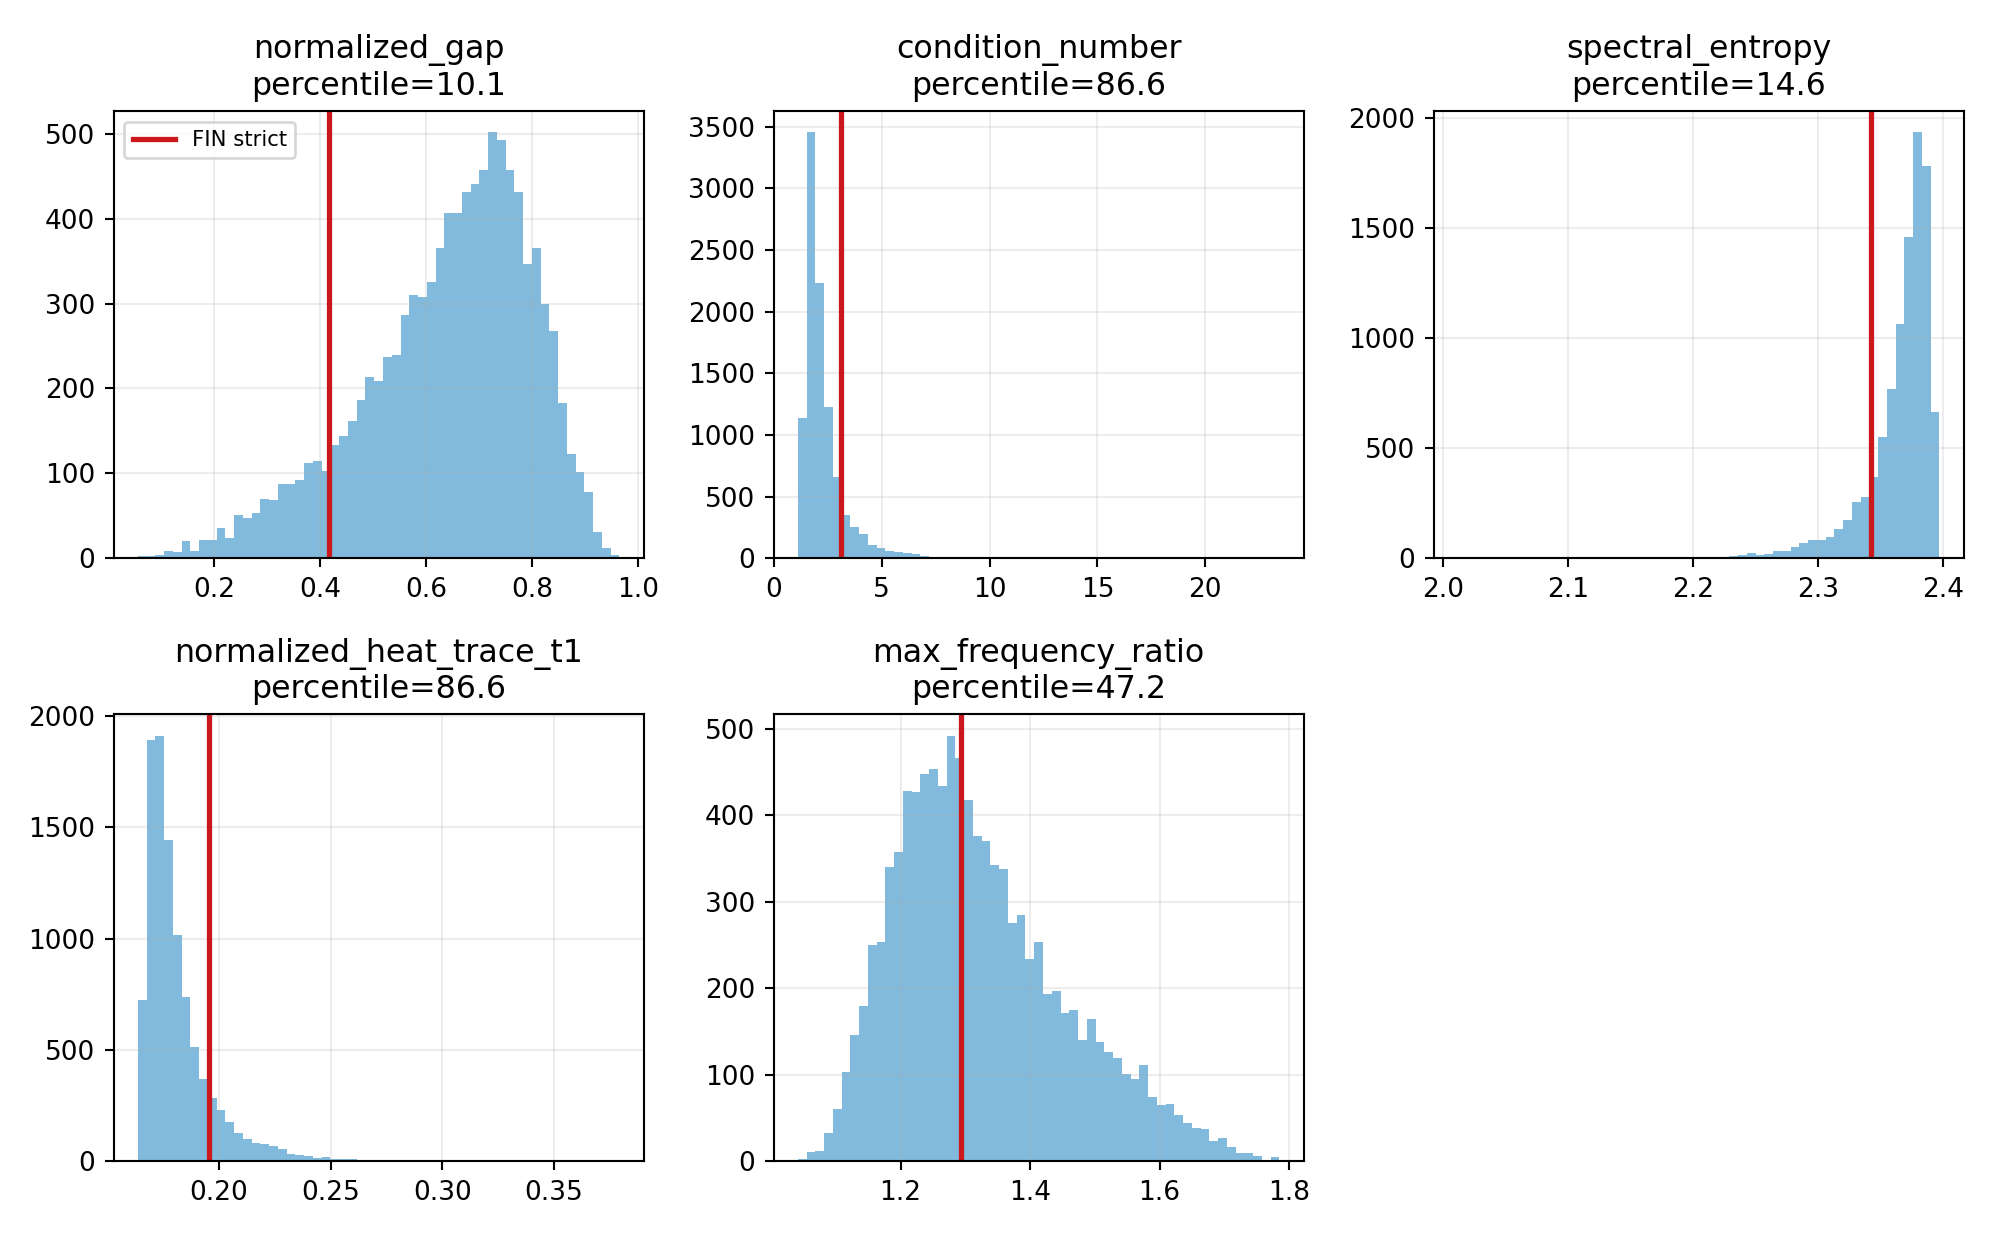
\includegraphics[width=0.93\textwidth]{FIN_TOE_Shadow_Atlas_Figures/positive_circulant_null_ensemble.png}
\caption{Pozycja strict w zadanym zespole lognormalnym. Wspólny rachunek funkcyjny jest generyczny w tej klasie; szczególna teoria wymaga dodatkowego niezmiennika lub predykcji.}
\end{figure}

\claimbox{\textbf{Wniosek falsyfikacyjny.} Wspólny rachunek funkcyjny jest realną unifikacją matematyczną, lecz nie odróżnia FIN od badanej klasy dodatnich radialnych laplasjanów. Kandydat na podpis FIN musi używać bardziej specyficznej struktury: zamrożonego profilu, relacji legacy--strict, dynamiki nieliniowej, reguły adaptacji, refinacji lub wspólnej wielosektorowej predykcji. ST03 rozszerza klasę kontroli.}

\section{Znane teorie jako objawy FIN: mapa zbiorcza}

\small
\begin{longtable}{@{}p{0.19\textwidth}p{0.25\textwidth}p{0.13\textwidth}p{0.34\textwidth}@{}}
\caption{Aktualny poziom relacji przy przyjęciu $H_{\rm TOE}$.}\\
\toprule
Teoria & Kandydacki cień FIN & Poziom & Najkrótszy brak\\
\midrule
\endfirsthead
\toprule
Teoria & Kandydacki cień FIN & Poziom & Najkrótszy brak\\
\midrule
\endhead
Spektralna teoria grafów & $A=sI-W$, Fourier na $C_{12}$ & E1/L1 & Fizyczna interpretacja nośnika\\
Teoria informacji & Shannon, data processing, Schur & E1/L1 & Ontologia informacji i skala energii\\
Dyfuzja Markowa & $e^{-tA}$ & E1/L1 & Zegar i identyfikacja stanów\\
Mechanika kwantowa & $e^{-itA}$ & E2/L1 & Born, $\hbar$, tensor products, pomiar\\
Green/odpowiedź & $(A+zI)^{-1}$ & E1/L1 & Fizyczne źródło i pole\\
Skończony model gaussowski & $S=\frac12\phi^TA\phi-J^T\phi$ & E2/L1 & Continuum, Lorentz, Fock, lokalność\\
Statystyka & $e^{-\beta A}/Z$ & E2/L1 & Energia, temperatura, kąpiel\\
Układy otwarte & Schur/Stieltjes, combs & E2/L1 & CPTP, środowisko, temporal realization\\
DNLS & $i\dot\psi=A\psi-|\psi|^2\psi$ & E2/L1 & FIN-owe źródło nieliniowości i skali\\
EFT/RG & Schur jako eliminacja gaussowska & E1(Schur), E3(RG)/L1 & Rodzina skal i przepływ beta\\
Mechanika klasyczna & współrzędne kolektywne & E3/L0 & Forma symplektyczna i limit klasyczny\\
Hydrodynamika/\newline solitony & lokalizowane fale nieliniowe & E3/L0 & PDE, prawa zachowania, travelling soliton\\
NCG & skończone dane spektralne & E3/L0--1 & Pełny triple, $J,\gamma$, działanie, cutoff\\
Tensor networks & hierarchiczna kompresja & E3/L0 & Tensory, izometrie, splątanie\\
Causal sets & skończony nośnik & E0/L0 & Porządek częściowy i Lorentzowski limit\\
Yang--Mills & fazy grafowe jako receiver & E0/L0 & Połączenie, krzywizna, grupa lokalna\\
Ogólna względność & widmo jako analog geometrii & E3/L0 & Metryka Lorentza, EH, dyfeomorfizmy\\
Model Standardowy & historyczne role węzłów & E0/L0 & Grupa, chiralność, anomalie, masy\\
\bottomrule
\end{longtable}
\normalsize

\begin{figure}[H]
\centering
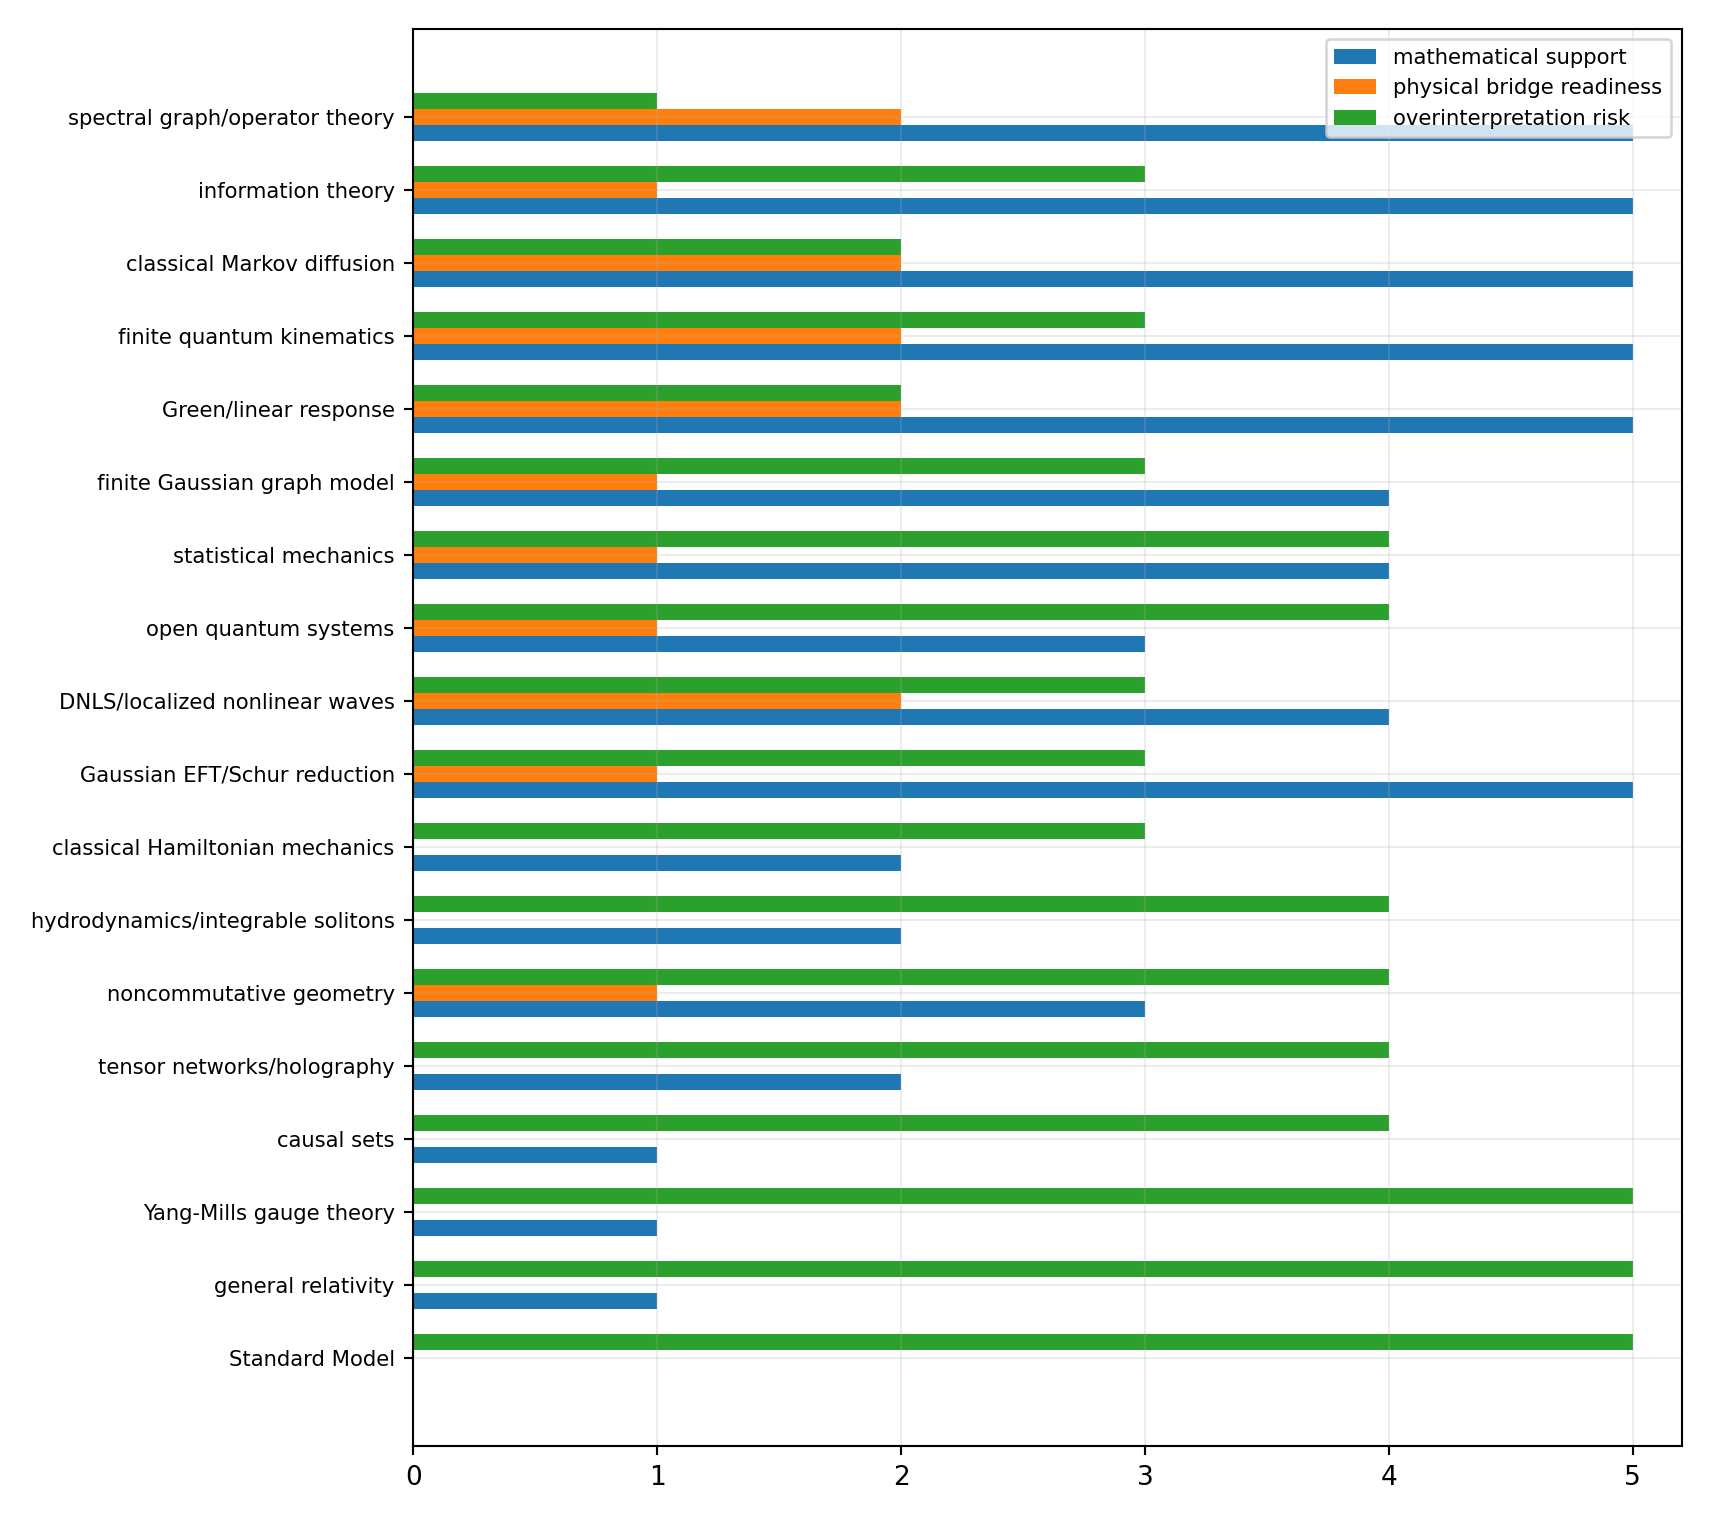
\includegraphics[width=0.89\textwidth]{FIN_TOE_Shadow_Atlas_Figures/theory_shadow_maturity_map.png}
\caption{Wsparcie matematyczne, gotowość mostu fizycznego i ryzyko nadinterpretacji. Skala 0--5 jest eksperckim porządkiem ordinalnym (0: brak, 5: najwyższy poziom w danej osi), a nie wynikiem twierdzenia ani prawdopodobieństwem.}
\end{figure}

\section{Mechanika kwantowa, klasyczna i dyfuzja}

\subsection{Skończona mechanika kwantowa}

Równanie Schrödingera
\[
i\hbar\partial_t\psi=H\psi
\]
otrzymuje reprezentację FIN po zadaniu $H=E_*A$, $t_{\rm phys}=\tau_*t$ i warunku $E_*\tau_*/\hbar=1$ \cite{Schrodinger}. Unitarność, interferencja i zachowanie normy są dokładne. Ciągły spacer kwantowy na grafie jest kanonicznym precedensem tej interpretacji \cite{FarhiGutmann}.

Nie wynika reguła Borna, ontologia amplitudy, kompozycja układów, algebra wszystkich obserwabli, przygotowanie, POVM ani $\hbar$. Obecne testery FIN typują te obiekty warunkowo, ale nie generują ich z $A$.

\textbf{Falsifier warunkowy.} Najpierw trzeba niezależnie zadeklarować przygotowania, instrumenty, regułę Borna i kalibrację czasu. Następnie tomografia fazowa i rozkłady przejścia powinny wyznaczyć klasy dopuszczalnych generatorów, uwzględniające globalne przesunięcie energii, skalę czasu i aliasing. Pusty przekrój tych klas odrzuca realizację kwantową $H_{1A}$; sama tomografia nie wyprowadza brakującej semantyki pomiaru.

\subsection{Dyfuzja i proces Markowa}

Ponieważ $A\mathbf1=0$ i $A_{xy}=-W_{xy}<0$ dla $x\ne y$, $-A$ jest generatorem procesu Markowa rewersyjnego względem miary jednostajnej (spełniającego szczegółową równowagę). Nie oznacza to odwracalności semigrupy dla ujemnego czasu. Dla $t=0.55$ minimum elementu $P_t$ wynosi $0.0122068$. Jest to dokładna konstrukcja probabilistyczna, lecz nadal nie fizyczne ciepło; tę samą własność ma każdy laplasjan z badanej dodatniej klasy zerowej.

\textbf{Falsifier.} Zamrożony model wymaga $P_{t+s}=P_tP_s$, niezmienniczej miary jednostajnej i tych samych szybkości $\lambda_r$, które pojawiają się w kanale koherentnym.

\subsection{Mechanika klasyczna}

Równania Hamiltona wymagają przestrzeni fazowej, formy symplektycznej i nawiasu Poissona. Lokalizowane profile mogą dostarczyć współrzędnych kolektywnych, ale repozytorium nie ma kontrolowanego limitu
\[
\{q_i,p_j\}=\delta_{ij},\qquad
\dot q_i=\partial_{p_i}H,\quad \dot p_i=-\partial_{q_i}H.
\]
Jest to program redukcji, nie obecny cień E1.

\section{Fale, hydrodynamika i nadsoliton}

Dodatni $A$ generuje równanie falowe
\[
\ddot\phi+A\phi=0,\qquad
\phi(t)=\cos(t\sqrt A)\phi_0+g_t(A)\dot\phi_0,
\]
gdzie rachunek funkcyjny obsługuje mod zerowy bez użycia nieistniejącego $A^{-1/2}$:
\[
g_t(\lambda)=
\begin{cases}
\sin(t\sqrt\lambda)/\sqrt\lambda,&\lambda>0,\\
t,&\lambda=0.
\end{cases}
\]
Wspólne widmo wyjaśnia, dlaczego ten sam fundament może wyglądać jak koherentna fala albo jak dyfuzja. Nie dostarcza prędkości światła, lokalnego stożka, metryki ani warunków brzegowych.

Częstości modów mogą definiować wewnętrzny czas fazowy i jego bezwymiarowe stosunki, co formalizuje intuicję ``soliton niesie zegar''. Nie wybierają jednak sekundy. Dla faz unitarnych zachodzi niezmienniczość
\[
(A,t_U)\longmapsto(cA,t_U/c),\qquad c>0,
\]
która zachowuje $e^{-it_UA}$; P522 dowodzi tej obstrukcji orbity skali dla ścisłego torusa częstości $\lambda_r$. Dla równania falowego osobna niezmienniczość ma postać $(A,t_C)\mapsto(cA,t_C/\sqrt c)$ i zachowuje $\cos(t_C\sqrt A)$. Żadna z nich nie jest twierdzeniem o nieprzeskalowanym DNLS. Zatem częstość może dać porządek i względny zegar w określonym sektorze, lecz absolutna jednostka czasu wymaga dodatkowego mostu wymiarowego.

Warunkowy DNLS
\[
i\dot\psi=A\psi-|\psi|^2\psi
\]
ma certyfikowaną gałąź lokalizowaną i granicę stabilności VK. P527 daje najmniejszy mechanizm znaku: dodatni mediator $B>0$ sprzężony z $\rho=|\psi|^2$ po eliminacji generuje
\[
-\frac{g^2}{2}\langle\rho,B^{-1}\rho\rangle.
\]
FIN nie wyprowadził jeszcze mediatora, $g^2/b$, nasycenia ani jego prawa czasowego. P531 wyklucza dokładny liniowo translacyjny stan o IPR $>1/8$, a skan nieliniowy nie znalazł kandydata. Termin ``soliton'' pozostaje hipotezą ontologiczną wspartą lokalizacją, nie pełnym twierdzeniem o solitonach w sensie Zabusky'ego--Kruskala \cite{ZabuskyKruskal}.

Samo zapisanie równania falowego lub DNLS nie jest podpisem FIN: oba można zbudować dla dowolnego odpowiedniego operatora PSD. Specyficzność wymaga bezrefitowej obserwabli zależnej od zamrożonego profilu strict i kontroli na alternatywnych operatorach.

Hydrodynamiczne nazwy ``lepkość'', ``prąd'' i ``turbulencja'' w dawnym diagramie nie są równaniami Naviera--Stokesa lub KdV. Aby taki cień powstał, potrzebne są pola zachowane, relacje konstytutywne, limit kontinuum i odpowiednie PDE.

\section{Green, QFT i teoria pól}

Dla działania gaussowskiego
\[
S_0[\phi,J]=\frac12\langle\phi,(A+m^2I)\phi\rangle-\langle J,\phi\rangle
\]
dla $m^2>0$ punkt stacjonarny i dwupunktowa kowariancja skończonego modelu gaussowskiego na grafie używają
\[
G_m=(A+m^2I)^{-1}.
\]
Dla $m=0$ trzeba usunąć mod stały, uziemić graf albo użyć pseudoodwrotności z dodatkowymi warunkami. Kandydatem na kowariancję/Green jest $G_m$, nie macierz sprzężeń $W=K_{\rm strict}$.

Pełna QFT wymaga jednak:
\begin{itemize}
\item rodziny lokalnych algebr lub pól operatorowych i struktury Focka;
\item CCR/CAR i statystyki bozonowej/fermionowej;
\item próżni, mikroprzyczynowości i sygnatury Lorentza;
\item refleksyjnej dodatniości dla rekonstrukcji Osterwaldera--Schradera \cite{OsterwalderSchrader};
\item refinacji $N\to\infty$, renormalizacji i stabilnych korelatorów.
\end{itemize}
Skończona rezolwenta nie jest automatycznie euklidesową funkcją Greena continuum, propagatorem Feynmana, propagatorem retarded ani potencjałem Yukawy. Obiekty te różnią się sygnaturą i warunkami brzegowymi. Nazwa ``Yukawa-type'' klasyfikuje kształt odpowiedzi po dodatkowych założeniach, nie wyprowadza pola fizycznego.

\textbf{Falsifier.} Należy skonstruować rodzinę FIN$_N$, wykazać zbieżność rezolwent i korelatorów, a następnie porównać bez refitu kilka funkcji n-punktowych.

\section{Układy otwarte i paradoks obserwatora}

Równanie Lindblada ma postać \cite{Lindblad,GKS}
\[
\dot\rho=-i[H,\rho]+\sum_k\left(L_k\rho L_k^\dagger-\frac12\{L_k^\dagger L_k,\rho\}\right).
\]
Istnienie $e^{-itA}$ i $e^{-tA}$ nie znaczy, że akt obserwacji przekształca pierwsze w drugie. $e^{-tA}$ działające na wektory klasycznych populacji nie jest automatycznie kanałem CPTP na macierzach gęstości.

Schur/Feshbach/Mori--Zwanzig pokazuje, jak ukryte stopnie swobody tworzą samoenergię
\[
\Sigma_E(z)=A_{EH}(zI+A_{HH})^{-1}A_{HE}
\]
i pamięć. P530 dowiódł kluczowej niejednoznaczności: ten sam operator zerowej częstotliwości dopuszcza różne realizacje czasowe. Odmienność ich stabilności ma status mocnego wyniku numerycznego dla zadanych rodzin i próbkowanych prędkości, a nie ogólnego twierdzenia Kreina. Proces tensorowy lub comb jest dobrym językiem brakującej struktury obserwatora, ale środowisko, instrument i rekord są dodatkowymi obiektami.

\textbf{Falsifier.} Trzeba sprawdzić całkowitą dodatniość, zachowanie śladu, tomografię wieloczasową i niezależny zapis zdarzeń. Sama ilustracja double slit nie wystarcza.

\section{Informacja, termodynamika i mechanika statystyczna}

Shannonowskie
\[
H(p)=-\sum_ip_i\log p_i
\]
jest dokładną miarą informacji \cite{Shannon}. Historyczna normalizacja warstwy legacy/scalar-shape $\alpha_{\rm geo}=4\ln2=\ln16$ jest liczbowo równa entropii w natach rozkładu jednostajnego na szesnastu stanach, \emph{jeśli} nada się jej tę interpretację. Sama równość nie ustanawia ani entropijnego pochodzenia $\alpha_{\rm geo}$, ani prawa fizycznego, ani transferu tej roli do strict. Nie oznacza też czterech jednostek energii.

Formalny stan Gibbsa
\[
\rho_\beta=\frac{e^{-\beta E_*A}}{Z},\qquad F=-\beta^{-1}\log Z
\]
jest dobrze zdefiniowany po dodaniu $E_*$ i $\beta$. Dla każdego dodatniego $p_i$ istnieje nieskończenie wiele par skal energii i temperatury
\[
E_i=-\theta\log p_i+C,qquad \beta=\theta^{-1}.
\]
Jaynesowska rekonstrukcja maksymalnej entropii \cite{Jaynes} wybiera rozkład pod zadanymi ograniczeniami; nie tworzy fizycznego Hamiltonianu z samego Shannona. Zasada Landauera \cite{Landauer} wymaga kąpieli, temperatury i procesu kasowania.

\begin{theorem}[Nieidentyfikowalność skali energia--temperatura]
Bezwymiarowy rozkład lub modularny Hamiltonian $-\log\rho$ nie wybiera osobno energii i temperatury. Jednoczesna transformacja $E\mapsto cE$, $\beta\mapsto\beta/c$ zachowuje wszystkie wagi.
\end{theorem}

Brak skali działania jest odrębną obstrukcją jednostkową: bezwymiarowe dane FIN pozostają niezmienione przy zmianie jednostki działania, więc wartość $\hbar$ albo równoważna stała musi pochodzić z dodatkowej mapy wymiarowej. Nie wynika to z samej transformacji Gibbsa.

Jeżeli FIN jest TOE, termodynamika byłaby cieniem dostępnej informacji po wyborze Hamiltonianu, kąpieli i skali, a nie prostym utożsamieniem ``bit = energia''.

\section{Renormalizacja, EFT i kompresja fraktalna}

Dokładna eliminacja dla $z>0$ używa dopełnienia Schura
\[
S_E(z)=A_{EE}+zI-A_{EH}(A_{HH}+zI)^{-1}A_{HE},
\qquad [(A+zI)^{-1}]_{EE}=S_E(z)^{-1}.
\]
Jest to skończony odpowiednik gaussowskiego całkowania po ukrytych zmiennych i dokładnie zachowuje przesuniętą odpowiedź Greena na widzialnym podukładzie. Przy $z=0$ osobliwy laplasjan wymaga odwracalności bloku, uziemienia, ograniczenia do $\mathbf1^\perp$ albo kontrolowanej pseudoodwrotności. Iteracja Schura daje kompozycyjną hierarchię opisów, ale jest generyczną eliminacją gaussowską. Fraktalna kompresja wymaga dodatkowo samopodobnej rodziny refinacji, prawa rekurencji i kontroli błędu; nie wynika z pojedynczego dopełnienia.

Pełne RG Wilsona \cite{Wilson} wymaga jednak parametru skali $\mu$, rodziny przestrzeni, przepływu sprzężeń
\[
\mu\frac{dg_i}{d\mu}=\beta_i(g),
\]
punktu stałego, uniwersalnych wykładników i odporności na schemat blokowania. FIN nie ma jeszcze kanonicznej rodziny $N\to\infty$. Powtarzany Schur daje skale względne, nie długość Plancka. ``Trzydzieści warstw fraktalnych'' i Planck endpoint pozostają historycznym zewnętrznym kotwiczeniem.

\textbf{Falsifier.} Dwa niezależne schematy blokowania muszą prowadzić do tych samych wykładników i korelatorów po wspólnej kalibracji. Brak zgodności obala uniwersalność, choć nie tożsamość Schura.

\section{Najwyższy rezonans a najniższa energia}

Dla
\[
A=sI-W
\]
wartości własne spełniają
\[
\lambda_j(A)=s-\mu_j(W).
\]
W obliczeniu błąd tej relacji wynosi $1.78\times10^{-15}$. Zatem
\[
\arg\max_j\mu_j(W)=\arg\min_j\lambda_j(A).
\]

Jeśli \emph{zdefiniuje się} siłę ``rezonansu'' jako wartość własną $\mu_j(W)$, a $A$ zinterpretuje jako energię, maksymalizacja tak rozumianego rezonansu jest równoważna minimalizacji $A$. Nie jest to twierdzenie o rezonansie wymuszonym w standardowym sensie fizycznym. Ponieważ $W$ ma dodatnie wagi, trybem Perrona--Frobeniusa o największej wartości własnej jest tutaj tryb jednostajny, a nie zlokalizowany nadsoliton. Nowa treść pojawiłaby się dopiero wtedy, gdy układ wybierałby stabilny rezonans wzbudzony przez gain, nasycenie i ograniczenia, którego nie można przepisać jako minimum przesuniętego operatora.

\section{Teorie cechowania i Model Standardowy}

Yang--Mills wymaga lokalnego połączenia i krzywizny \cite{YangMills}
\[
F_{\mu\nu}=\partial_\mu A_\nu-\partial_\nu A_\mu+[A_\mu,A_\nu],
\qquad D_\mu F^{\mu\nu}=J^\nu.
\]
Realny radialny kernel FIN nie zawiera zmiennych łączowych $U_{xy}$, lokalnego działania $G^V$, prawa Gaussa, pętli Wilsona ani nieabelowego komutatora. Fazy i chiralne odbiorniki pokazują, gdzie taki sektor mógłby się sprzęgać, lecz nie są nim.

Warunkowe DNLS ma globalną symetrię $U(1)$, lecz globalna zmiana fazy nie jest lokalnym cechowaniem. Nieprzemienny komutant wynikający z degeneracji $A$ również nie dostarcza sam z siebie połączenia, holonomii ani krzywizny.

Model Standardowy wymaga grupy $SU(3)\times SU(2)\times U(1)$, reprezentacji chiralnych, anulowania anomalii, trzech generacji, Higgsa, Yukaw i parametrów \cite{Weinberg}. Obecne sloty receiver/scaffold nie są źródłem tych struktur. Dawne przypisania węzłów, $\sin^2\theta_W=\alpha_{\rm geo}/12$, wzór na $\alpha_{\rm EM}$ i hierarchia $\beta^N$ nie mogą przejść na strict bez pełnego completion i osobnego role-transfer theorem.

\textbf{Falsifier.} Bez dopasowania należy wyprowadzić grupę, reprezentacje, anomalie i co najmniej jeden nowy stosunek obserwabli. Inaczej FIN jest co najwyżej pojemnym receiverem.

\section{Grawitacja i geometria emergentna}

Widmo laplasjanu może kodować część geometrii, a w rodzinach continuum ślad cieplny ma rozwinięcia geometryczne. Widmo nie wyznacza jednak geometrii jednoznacznie: istnieją nieizometryczne obiekty izospektralne \cite{GordonWebbWolpert}. Pojedyncza macierz $12\times12$ nie ma asymptotyki Weyla ani lokalnego szeregu współczynników Seeley--DeWitta. Tym bardziej nie daje metryki Lorentza, stożków świetlnych, zasady równoważności, dyfeomorfizmów, tensora energii-pędu ani działania Einsteina--Hilberta \cite{Einstein}.

Programy emergentnej grawitacji, na przykład termodynamiczne równanie Einsteina Jacobsona \cite{Jacobson}, pokazują, że równania grawitacji mogą wynikać z dodatkowej struktury termodynamicznej. Nie dowodzą, że dowolna entropia lub graf FIN automatycznie daje GR. Pełne sprzężenie strict powoduje natychmiastowe niezerowe amplitudy między wszystkimi wierzchołkami, więc nie istnieje dokładny lokalny stożek przyczynowy.

\textbf{Falsifier.} Potrzebna jest rodzina refinacji z sygnaturą Lorentza, kontrolowanym limitem propagacji oraz zanikającym residualem równań Einsteina dla więcej niż jednej geometrii.

\section{Geometria nieprzemienna}

Tryplet spektralny $(\mathcal A,\mathcal H,D)$ i działanie
\[
S_{\rm spec}=\operatorname{Tr}f(D/\Lambda)+\langle\psi,D\psi\rangle
\]
są naturalnym porównaniem \cite{ChamseddineConnes}. FIN posiada $\mathcal H$ i operator spektralny, ale $A$ nie jest automatycznie operatorem Diraca. Brakuje kanonicznej algebry, reprezentacji, struktury rzeczywistej $J$, gradacji $\gamma$, aksjomatu pierwszego rzędu, orientowalności i wymiaru. Samo działanie spektralne zawiera cutoff $\Lambda$; nie rozwiązuje problemu skali.

NCG może być językiem przyszłego rozszerzenia \eqref{eq:extendedfin}. Obecnie jest analogią E3, ponieważ wiele nieizomorficznych trypletów pasuje do tej samej macierzy.

\section{Causal sets, tensor networks i holografia}

Causal set jest lokalnie skończonym porządkiem częściowym $(C,\prec)$ \cite{Bombelli}. Nieskierowany pełny graf wagowy na $C_{12}$ nie ma antysymetrycznej i przechodniej relacji przyszłość--przeszłość. Skierowany cykl również nie jest porządkiem przyczynowym. Prymitywy są obecnie niezgodne.

Tensor networks i MERA opisują faktoryzację przestrzeni Hilberta, izometrie i wieloskalowe splątanie \cite{Vidal,Swingle}. Schur przypomina hierarchiczną kompresję, lecz nie konstruuje tensorów, disentanglerów ani prawa entanglement entropy. Holografia AdS/CFT wymaga słownika bulk--boundary i zgodności korelatorów \cite{Maldacena}; żadna taka dualność nie została wyprowadzona z FIN.

\textbf{Falsifier.} Dla tensorowego cienia trzeba jawnie zbudować lokalne tensory i kontrolować błąd obcięcia. Dla causal set należy wyprowadzić porządek i continuum approximation. Słowa ``fraktalny'' i ``holograficzny'' nie zastępują tych konstrukcji.

\section{Samouczenie, sieci neuronowe i bootstrap}

Macierz $W$ przypomina warstwę neural operator, a przepływ
\[
\dot K=-\Pi\bigl(V'(K)-C(K)\bigr)
\]
może być gradientowym prawem adaptacji. Dla ustalonego celu istnieją twierdzenia Lyapunova. Zamrożony kernel jednak się nie uczy; funkcja celu, dane, aktualizacja i źródło feedbacku są dodatkowymi strukturami.

Ta sama postać gradientowa może zostać narzucona niemal dowolnemu operatorowi. Kontrolą negatywną musi być rodzina alternatywnych $W$ z identycznym budżetem parametrów; znaczenie FIN miałaby dopiero przewaga predykcyjna zamrożonej reguły bez strojenia celu po wyniku.

Pod $H_{\rm TOE}$ sensowna narracja brzmi: obserwowane prawa są stabilnymi punktami adaptacyjnego operatora informacji. Aby stała się teorią, trzeba wykazać integrability pola uczenia, jego pochodzenie z FIN, stabilność i unikatowość. P536 dowodzi, że skończone rekordy wybierają jedynie klasę praw modulo jądro mapy rekordowej, a rozkład posterior na niewidzialnym włóknie dziedziczy prior.

\section{Czy materia i światło mogą być cieniami?}

\textbf{Światło.} Koherentne bezmasowe lub niskoenergetyczne mody są matematycznie reprezentowalne, lecz ma je także szeroka klasa operatorów PSD. Brakuje Lorentzowskiej dyspersji, dwóch polaryzacji, lokalnej symetrii $U(1)$, ładunków i prędkości $c$. Status: \analogy{}.

\textbf{Materia.} Warunkowa nieliniowość może stabilizować lokalizowane profile. Nie ma jeszcze spin/statystyki, sektora topologicznego na refinacji, masy, reprezentacji gauge ani trwałych zderzeń. Status: \conditional{} dla lokalizacji, \absent{} dla cząstek Modelu Standardowego.

\textbf{Obserwator.} Procesy, combs, instrumenty i rejestry są formalnie zbudowane downstream. Nie wynikają z samego operatora. Status: \conditional{}.

Zatem porządek nadsoliton $\to$ światło $\to$ materia $\to$ obserwator pozostaje spójnym programem konstrukcyjnym. Nie jest jeszcze łańcuchem twierdzeń.

\section{Najbardziej mylące podobieństwa}

\begin{longtable}{@{}p{0.27\textwidth}p{0.31\textwidth}p{0.33\textwidth}@{}}
\toprule
Podobieństwo & Dlaczego przekonuje & Dlaczego nie wystarcza\\
\midrule
Kernel Yukawy & tłumiona odpowiedź/rezolwenta & brak pola Lorentza, masy i continuum\\
Shannon = entropia & ten sam logarytm & brak $k_B,T,H$ i procesu\\
$C_{12}$ = dwanaście oktaw & czytelna okresowość & liczba 12 nie wybiera sektorów fizycznych\\
warstwy fraktalne = Planck & hierarchia skal & Planck jest zewnętrznym kotwiczeniem\\
double slit = QM FIN & interferencja występuje & generuje ją każdy unitarny operator\\
unitary/diffusion = pomiar & dwa kanały z jednego $A$ & brak CPTP instrumentu i rekordu\\
spectral triple = NCG fizyczna & pasuje język widmowy & triple i jego aksjomaty nie są unikatowe\\
adaptacja = uczący się wszechświat & istnieje flow gradientowy & cel i feedback są dostarczone\\
najwyższy rezonans = nowe prawo & intuicyjna odmienność & dla $A=sI-W$ to minimum $A$\\
\bottomrule
\end{longtable}

\section{Co wynika, jeśli mimo wszystko hipoteza TOE jest prawdziwa?}

Jeśli hipoteza jest prawdziwa, znane teorie nie są ``błędne''. Są stabilnymi opisami różnych funktorów obserwacyjnych:
\begin{itemize}
\item QM zachowuje fazę i pełną koherencję wybranego sektora;
\item dynamika Markowa traci fazę i śledzi populacje;
\item termodynamika opisuje maksymalnie skompresowane rozkłady z ograniczeniami;
\item QFT byłaby limitem kontinuum korelatorów i propagatorów;
\item GR opisywałaby geometrię efektywnej propagacji i przyczynowości;
\item gauge theory opisywałaby lokalne porównanie faz między kontekstami;
\item RG opisywałoby zmianę prawa przy usuwaniu informacji ukrytej;
\item solitony i materia byłyby stabilnymi nieliniowymi sektorami tej samej informacji;
\item obserwator byłby częścią operacyjnego podziału widzialne--ukryte i zapisu.
\end{itemize}

To jest spójny obraz syntezy, ale każda strzałka wymaga oddzielnego twierdzenia \eqref{eq:intertwine}. $H_{\rm TOE}$ nie opłaca map przez samo założenie.

\section{Kryteria rzeczywistej TOE}

FIN zasługiwałby na fizyczne miano TOE dopiero po spełnieniu łącznie:
\begin{enumerate}
\item jednego wspólnego ścisłego rdzenia i niesprzecznych sektorów;
\item przestrzeni stanów, algebry obserwabli i prawa składania układów;
\item selektora lub jawnego aksjomatu sektora;
\item źródła skali długości, czasu i działania;
\item probabilistyki oraz teorii pomiaru;
\item kontrolowanej refinacji i limitu kontinuum;
\item wyprowadzenia lokalności, przyczynowości i symetrii czasoprzestrzeni;
\item wspólnego źródła parametrów co najmniej kilku sektorów;
\item zgodności diagramów w obszarach nakładania, np. FIN$\to$QFT$\to$QM i FIN$\to$QM;
\item co najmniej jednej nowej predykcji odróżniającej FIN od zespołu zerowego.
\end{enumerate}

Bez punktu dziesiątego nawet kompletna reinterpretacja może nie być empirycznie wyróżniona.

\section{Programy dalsze ST01--ST15}

Wszystkie poniższe prace można rozpocząć lokalnie, analitycznie lub obliczeniowo.

\begin{longtable}{@{}p{0.07\textwidth}p{0.11\textwidth}p{0.71\textwidth}@{}}
\toprule
ID & Priorytet & Zadanie i kryterium sukcesu\\
\midrule
ST01 & 1 & \textbf{Shadow Theorem Packet}: sformalizować L0--L5, mapy \eqref{eq:shadowdiagram} i warunki komutowania; każda przyszła identyfikacja musi dostarczyć certyfikat.\\
ST02 & 2 & \textbf{Common Spectrum Consistency}: zaprojektować jednoczesną rekonstrukcję $A$ z kanałów unitary/heat/Green/Gibbs przy zamrożonych skalach i kontrolach aliasingu.\\
ST03 & 3 & \textbf{Generic-Operator Null Atlas}: rozszerzyć kontrolę zerową na izospektralne, nieradialne, losowe PSD i signed-kernel ensembles; znaleźć statystykę naprawdę specyficzną dla FIN.\\
ST04 & 4 & \textbf{Algebra Completion}: sklasyfikować minimalne generatory $B_j$, dla których $C^*(A,B_1,\ldots)=M_{12}$, oraz sprawdzić ich pochodzenie i symetrie.\\
ST05 & 5 & \textbf{Continuum Family Obstruction}: udowodnić istnienie kanonicznej rodziny FIN$_N$ albo no-go dla QFT/GR na poziomie L3.\\
ST06 & 6 & \textbf{Lorentzian Audit}: testować skończoną prędkość propagacji, sygnaturę i stożki; pełne sprzężenie jest kontrolą negatywną.\\
ST07 & 7 & \textbf{Information--Thermodynamics Bridge}: wyznaczyć minimalny zbiór $(\rho,H,\beta,\mathcal P,E_*)$ i dowieść konieczności każdego elementu.\\
ST08 & 8 & \textbf{Gauge-Holonomy Candidate}: dodać jawne link variables, a następnie sprawdzić, czy grupa, prawo Gaussa i Ward identities wynikają, czy zostały przepisane.\\
ST09 & 9 & \textbf{Saturating Mediator}: domknąć P527 potencjałem ograniczonym z dołu i udowodnić stabilność globalną bez dopasowania do oczekiwanego solitonu.\\
ST10 & 10 & \textbf{Memory Krein Theorem}: rozstrzygnąć dokładnie stabilność hamiltonowskiej realizacji pamięci P530 i porównać z klasą relaksacyjną.\\
ST11 & 11 & \textbf{RG Scheme Independence}: dwie różne hierarchie Schura muszą dać te same niezmienniki i wykładniki albo hipoteza fraktalnego fixed point odpada.\\
ST12 & 12 & \textbf{Legacy--Strict Role Matrix}: dopiero po completion ocenić osobno każdą dawną rolę EW, EM, hierarchii i fazy; obecnie zachować zakaz transferu.\\
ST13 & 13 & \textbf{Cross-Theory Frozen Parameters}: jedna kalibracja FIN, następnie bez refitu test kanałów koherentnego, dyfuzyjnego, termicznego i odpowiedzi.\\
ST14 & 14 & \textbf{Prediction Ledger}: zamrozić jedną obserwablę nieposiadaną przez null ensemble, kryterium falsyfikacji i hash przed obliczeniem hold-out.\\
ST15 & 15 & \textbf{Formal Core}: sformalizować Dirichleta, wspólne widmo, Schur, no-go skali, no-go selektora i obstrukcję $C^*(A)$ w jednym pakiecie.\\
\bottomrule
\end{longtable}

\section{Werdykt końcowy}

Przy założeniu $H_{\rm TOE}$ najbardziej produktywna interpretacja brzmi:

\claimbox{FIN jest kandydatem na wspólny informacyjno-spektralny substrat, którego różne operacje --- zachowanie fazy, tłumienie, odwrócenie operatora, marginalizacja i nieliniowa odpowiedź --- mogą wyglądać na poziomie efektywnym jak różne znane prawa fizyki.}

Najsilniejsza część tego zdania jest już twierdzeniem matematycznym: unitary, heat, wave, Green i formal Gibbs są dokładnymi transformacjami jednego generatora, a przesunięty Schur zachowuje odpowiedni blok Greena. Nie są przez to automatycznie cieniami fizycznymi. Najsłabsza część dotyczy właśnie identyfikacji: nie wiadomo jeszcze, dlaczego konkretna transformacja ma być mechaniką kwantową, temperaturą, materią, cechowaniem lub czasoprzestrzenią.

Analiza nie znajduje sprzeczności wewnątrz zbadanej skończonej warstwy operatorowej. Nie może orzec spójności całego $H_{\rm TOE}$, ponieważ hipoteza nie definiuje jeszcze wszystkich sektorów ani map między nimi. Twarda granica brzmi: pojedynczy rachunek $C^*(A)$ tworzy wyłącznie przemienny atlas funkcji widma. TOE potrzebuje dodatkowej algebry, sektorów, skali, refinacji i operacyjnego rekordu. Jeżeli te obiekty zostaną wyprowadzone wspólnie i ich diagramy przejdą testy bez osobnego dopasowania, narracja ``znane teorie opisują po omacku FIN'' stanie się programem redukcji fizycznej. Dziś jest rygorystycznie uporządkowaną hipotezą, kilkoma dokładnymi transformacjami matematycznymi i wieloma jawnymi brakami.

\appendix
\section{Reprodukcja obliczeń}

\begin{verbatim}
sha256sum -c FIN_TOE_SHADOW_ATLAS_INPUTS.sha256
MPLCONFIGDIR=/tmp/fin-toe-mpl python3 fin_toe_shadow_atlas_analysis.py
python3 -m unittest -v test_fin_toe_shadow_atlas.py
pdflatex -interaction=nonstopmode -halt-on-error \
  FIN_Hypothetical_TOE_Shadow_Atlas_Comparative_Report_PL.tex
\end{verbatim}

Pakiet obejmuje wyniki JSON, trzy wykresy, kod, jedenaście testów, skróty wejściowego snapshotu i manifest SHA-256. Plik \texttt{FIN\_TOE\_SHADOW\_ATLAS\_INPUTS.sha256} identyfikuje lokalne źródła użyte ponad bazowym HEAD; drzewo robocze nie było czyste. Wyszukiwanie internetowe służyło wyłącznie identyfikacji literatury pierwotnej; nie stanowi danych empirycznych FIN.

\section{Proweniencja wyników repozytoryjnych}

Odwołania do P522, P527, P530, P531 i P536 są jawnie oznaczonymi wynikami wcześniejszych pakietów repozytorium, a nie twierdzeniami ponownie dowiedzionymi w niniejszym skrypcie. Ich źródłami audytowalnymi są
\begin{itemize}
\item \texttt{FIN\_Programs\_517\_526\_Fourth\_Jet\_Stability\_and\_Clock\_Report\_EN.pdf} (P522),
\item \texttt{FIN\_Programs\_527\_536\_Auxiliary\_Field\_Memory\_and\_Exact\_Replay\_Report\_EN.pdf},
\item \texttt{FIN\_Programs\_527\_536\_Results.json},
\item \texttt{RELEASE\_10\_53\_PROGRAMS\_527\_536\_AUXILIARY\_FIELD\_MEMORY\_EXACT\_REPLAY.md}.
\end{itemize}
Niniejsza Release 10.54 niezależnie oblicza wyłącznie audyt operatora strict, zespół zerowy, diagnostyk legacy--strict i mapę porównawczą. Statusy wcześniejszych programów zachowują ich własne granice dowodowe.

\begin{thebibliography}{99}
\bibitem{Shannon} C. E. Shannon, \emph{A Mathematical Theory of Communication}, Bell System Technical Journal 27 (1948), \url{https://doi.org/10.1002/j.1538-7305.1948.tb01338.x}.
\bibitem{Landauer} R. Landauer, \emph{Irreversibility and Heat Generation in the Computing Process}, IBM Journal of Research and Development 5 (1961), \url{https://doi.org/10.1147/rd.53.0183}.
\bibitem{Jaynes} E. T. Jaynes, \emph{Information Theory and Statistical Mechanics}, Physical Review 106 (1957), \url{https://doi.org/10.1103/PhysRev.106.620}.
\bibitem{Lindblad} G. Lindblad, \emph{On the Generators of Quantum Dynamical Semigroups}, Communications in Mathematical Physics 48 (1976), \url{https://doi.org/10.1007/BF01608499}.
\bibitem{GKS} V. Gorini, A. Kossakowski, E. C. G. Sudarshan, \emph{Completely Positive Dynamical Semigroups of N-Level Systems}, Journal of Mathematical Physics 17 (1976), \url{https://doi.org/10.1063/1.522979}.
\bibitem{FarhiGutmann} E. Farhi, S. Gutmann, \emph{Quantum Computation and Decision Trees}, Physical Review A 58 (1998), \url{https://arxiv.org/abs/quant-ph/9706062}.
\bibitem{ZabuskyKruskal} N. J. Zabusky, M. D. Kruskal, \emph{Interaction of ``Solitons'' in a Collisionless Plasma and the Recurrence of Initial States}, Physical Review Letters 15 (1965), \url{https://doi.org/10.1103/PhysRevLett.15.240}.
\bibitem{Wilson} K. G. Wilson, \emph{The Renormalization Group: Critical Phenomena and the Kondo Problem}, Reviews of Modern Physics 47 (1975), \url{https://doi.org/10.1103/RevModPhys.47.773}.
\bibitem{YangMills} C. N. Yang, R. L. Mills, \emph{Conservation of Isotopic Spin and Isotopic Gauge Invariance}, Physical Review 96 (1954), \url{https://doi.org/10.1103/PhysRev.96.191}.
\bibitem{Weinberg} S. Weinberg, \emph{A Model of Leptons}, Physical Review Letters 19 (1967), \url{https://doi.org/10.1103/PhysRevLett.19.1264}.
\bibitem{ChamseddineConnes} A. H. Chamseddine, A. Connes, \emph{The Spectral Action Principle}, Communications in Mathematical Physics 186 (1997), \url{https://arxiv.org/abs/hep-th/9606001}.
\bibitem{Jacobson} T. Jacobson, \emph{Thermodynamics of Spacetime: The Einstein Equation of State}, Physical Review Letters 75 (1995), \url{https://arxiv.org/abs/gr-qc/9504004}.
\bibitem{Bombelli} L. Bombelli, J. Lee, D. Meyer, R. D. Sorkin, \emph{Space-Time as a Causal Set}, Physical Review Letters 59 (1987), \url{https://doi.org/10.1103/PhysRevLett.59.521}.
\bibitem{Vidal} G. Vidal, \emph{Entanglement Renormalization}, Physical Review Letters 99 (2007), \url{https://doi.org/10.1103/PhysRevLett.99.220405}.
\bibitem{Swingle} B. Swingle, \emph{Entanglement Renormalization and Holography}, Physical Review D 86 (2012), \url{https://arxiv.org/abs/0905.1317}.
\bibitem{Maldacena} J. Maldacena, \emph{The Large N Limit of Superconformal Field Theories and Supergravity}, Advances in Theoretical and Mathematical Physics 2 (1998), \url{https://arxiv.org/abs/hep-th/9711200}.
\bibitem{Schrodinger} E. Schrödinger, \emph{Quantisierung als Eigenwertproblem}, Annalen der Physik 384 (1926), \url{https://doi.org/10.1002/andp.19263840404}.
\bibitem{Einstein} A. Einstein, \emph{Die Grundlage der allgemeinen Relativitätstheorie}, Annalen der Physik 354 (1916), \url{https://doi.org/10.1002/andp.19163540702}.
\bibitem{OsterwalderSchrader} K. Osterwalder, R. Schrader, \emph{Axioms for Euclidean Green's Functions}, Communications in Mathematical Physics 31 (1973), \url{https://doi.org/10.1007/BF01645738}.
\bibitem{GordonWebbWolpert} C. Gordon, D. Webb, S. Wolpert, \emph{One Cannot Hear the Shape of a Drum}, Bulletin of the American Mathematical Society 27 (1992), \url{https://doi.org/10.1090/S0273-0979-1992-00289-6}.
\end{thebibliography}

\end{document}
